% !TeX root = ../main.tex

\chapter*{1. Introduction}
\setcounter{chapter}{1}
 \addcontentsline{toc}{chapter}{1. Introduction}
	\noindent
	Diverse ecological processes result in different species composition in the metacommunity across space and time. Ecologists have proposed several analytical methods to estimate the strength of these underlying processes to the variation of species composition. However, since in case of natural communities we can never know the real strength of these processes on the variation of species composition, those analytical methods are difficult to evaluate. One solution may be to draw support from the metacommunity simulation models. By using the community data which is simulated based on the known strength of ecological processes, we may evaluate whether the estimation derived by the analytical methods is correct or not. In our study, we use the simulated data to explore the behaviors of multiple analytical methods and to understand whether they can successfully estimate the strength of the ecological processes underlying the observed metacommunities.
	
	\section{Effects of multiple processes on metacommunity structure}
	\noindent
	Multiple ecological processes act in a metacommunity simultaneously across the spatial and temporal scales and result in the dynamics of the species composition. At a local scale, competition and ecological drift are the processes that may determine the local community structure \citep{leibold2004metacommunity}. Competition is a negative species interaction that describes the impact of the population size of a species on the growth rate of itself or the other species. The coexistence of the competing species may result from the differentiation in resource usage or the similarity in fitness (or carrying capacity) of the species \citep{macarthur1967limiting, chesson2000mechanisms}. In contrast, ecological drift is a stochastic process that describes the cause of demographical stochasticity or environmental stochasticity in the death of an individual or the extinction of a species within a local community \citep{hubbell2011unified}. After an individual dies, the space is released and the surrounding species may have a chance to establish in the space \citep{fukami2015historical}. At the regional scale, environmental filtering and dispersal may play the role in regulating the species turnover \citep{leibold2004metacommunity}. The species that do not tolerate given abiotic environmental conditions will be absent from the local community \citep{kraft2015community}. Different strengths of the dispersal ability of the species may alleviate or facilitate the flow of propagules between local communities \citep{tilman1997community, macarthur1967theory}. These ecological processes may interact with each other and simultaneously drive the species turnover across spatial and temporal scales \citep{thompson2020process}. Metacommunity archetypes are the different perspectives of the metacommunity and focus on different ecological processes \citep{leibold2004metacommunity, leibold2017metacommunity} (Tab. \ref{tbl:def}). 
	
	Predicting the future dynamics of the metacommunity structure under the pressure of anthropogenic activity and climate change has already become an essential topic in conservation \citep{clark2001ecological, evans2012modelling, chase2020biodiversity}. By studying the relationship between anthropogenic factors and climatic conditions to the strength of ecological processes across metacommunities, the mechanisms underlying the loss of ecosystem services may be disentangled. This may improve the management decisions to optimize ecosystem services \citep{hodgson2019investigating, chase2020biodiversity}. How to estimate the strength of ecological processes underlying the observed metacommunities becomes an urgent question that is related to human welfare.
	
	Process-based model is an approach to studying how the ecological processes would affect the species composition of a metacommunity. A process-based model is defined as “a model that characterizes changes in a system's state as explicit functions of the events that drive those state changes” \citep{connolly2017process}. It does not need to be deterministic, but it can also encompass stochastic ecological processes, such as demographic stochasticity and dispersal \citep{connolly2017process}. The parameters in the model may represent the strength of certain ecological processes. By altering the parameters within the process-based model, we may study the effect of the processes on species coexistence \citep{adler2007niche, adler2010coexistence} and the relative abundance of the species \citep{ke2015soil}. Moreover, by fitting the model parameters in the process-based model, the strength of the ecological processes underlying the observed metacommunity may be disentangled. For example, \citet{adler2010coexistence} fitted the process-based models by four plant species data from U.S. Sheep Experiment Station and proposed that stabilizing mechanisms are important to maintain the diversity of plant community. The strength of the processes may also be compared across metacommunities \citep{adler2018competition}.  
	
	
	\afterpage{
		\begin{footnotesize}
			\begin{longtable}{p{0.35\textwidth}p{0.6\textwidth}}
				\caption[Definition of the terms used in our study.]{\small
					Definition of the terms used in our study.}
				\label{tbl:def}
				\endfirsthead
				\toprule
				Term & Definition\\
				\midrule
				Species turnover & The changes in species composition across space and time.\\
				Metacommunity & A metacommunity is a set of local communities linked by the dispersal of multiple interacting species \citep{wilson1992complex, leibold2004metacommunity}. In our study, the observed metacommunity is defined as the metacommunity in the field, and the simulated metacommunity is the metacommunity generated by the simulation model.\\
				Ecological process & The force that drives the species turnover across space and time. In the metacommunity ecology framework, four high-level processes are proposed to drive species turnover: competition, ecological drift, environmental filtering and dispersal \citep{leibold2017metacommunity}.\\
				Metacommunity archetypes & Four metacommunity archetypes are the different perspectives to study the species turnover within the metacommunity \citep{leibold2004metacommunity, leibold2017metacommunity}:\\
				\hspace{1em} \textit{Patch dynamics} (PD) & Competition hierarchy and trade-off in competition and colonization ability among species determine the local extinction and colonization of the species and further cause the species turnover within the metacommunity.\\
				\hspace{1em} \textit{Species sorting} (SS) & Species interaction and demographic differences between species, which are associated with the environmental heterogeneity across space and time, are the main drivers of the species turnover within the metacommunity.\\
				\hspace{1em} \textit{Neutral dynamics} (ND) & Species in the metacommunity are demographically similar. Dispersal limitation among local communities and ecological drift caused by the demographic stochasticity within the local patches are the main drivers of species turnover.\\
				\hspace{1em} \textit{Mass effect} (ME) & The maladaptive species (the species that has weaker competitive ability or fitness compared to the other species) within the local community may maintain its population via strong dispersal inflow from the other communities and prevent it to be out-competed.\\
				Analytical methods & The analytical methods discussed in our study are the statistical approaches that summarize the ecological information based on the ecological community data by multiple summary statistics. The summary statistics may indicate the influence of certain ecological processes on species turnover. For example, beta-diversity variation partitioning is one of the analytical methods, that uses constrained ordination to relate species composition with environmental and geographical variables. The variation explained by environmental and geographical variables are the summary statistics of this method.\\
				Process-based simulation models & The process-based approach explicitly models the effect of ecological processes on the state of the system, e.g. population size. The parameters in the process-based model may regulate the strength of the ecological processes. By modifying the model parameters, we may study how species composition would be influenced by the ecological processes.\\
				\bottomrule
			\end{longtable}
		\end{footnotesize}
	}
	
	\section{Analytical methods to infer the underlying ecological processes}
	\noindent
	Ecologists have proposed analytical methods that aim to identify the presence (or quantify the relative importance) of the ecological processes since the mid of 20th century \citep{macarthur1958population, diamond1975island}. More recently, ecologists starts to integrate multiple types of data, e.g. data about the environmental conditions, functional traits and phylogeny, and propose various analytical methods to summarize the ecological information from the observed metacommunity by multiple summary statistics. These summary statistics were proposed to quantify the effect of certain ecological processes on the species turnover or variation in functional traits and phylogeny structure (Fig. \ref{fig:framework}a). 
	
	Null model is one of the approaches to comparing the observed community data to the one after randomization \citep{gotelli2006null, gotelli2012statistical}. The randomized data is assumed to be the one derived from a metacommunity without certain underlying processes, which is suggested to be the null hypothesis. If the observed data is far different from the randomized one, i.e. the null hypothesis is rejected, then the presence of the processes may be confirmed. Without the information on the habitat condition, studying the clustering or over-dispersion of the species composition may disentangle the effect of environmental filtering and competition on species turnover among local communities \citep{diamond1975island, connor1979assembly, chase2011disentangling}. On the other hand, testing the convergence or the divergence of the functional traits and phylogeny composition between communities may also identify whether the observed metacommunity is mainly driven by environmental filtering or competition \citep{mayfield2010opposing}. Null model approach may also quantify the relative importance of niche and dispersal processes underlying the metacommunity based on species composition and their phylogeny or functional traits \citep{stegen2013quantifying, ford2020functional}, or only based on species composition \citep{gibert2019per, vilmi2021dispersal}. Environmental and geographical data are dispensable for these null model-based analytical methods, which benefits the empiricists to apply these methods in practice. However, it is difficult to benchmark whether the algorithm of randomization correctly diminishes the effect of certain ecological processes. The mismatch between the algorithm and the null hypothesis may result in the wrong type I error rate of the hypothesis testing \citep{molina2020difficulties}.   
	
	Other analytical methods are based on the summary statistics derived from the correlation between different types of data, e.g. canonical analysis and hierarchical joint species distribution approach. By canonical analysis, species composition is regressed on environmental and geographical attributes \citep{borcard1992partialling}, or even functional traits and phylogeny structure within the local communities \citep{sirbu2021variation}. This approach is called beta-diversity variation partitioning in the following text. The relative importance of environmental filtering and dispersal may be estimated by the amount of compositional variation explained by environmental and geographical data \citep{cottenie2005integrating}. The hierarchical joint species distribution approach uses a hierarchical generalized linear model to relate species composition with environment, traits and phylogeny. In the hierarchical modeling of species community (HMSC) proposed by \citet{ovaskainen2017make}, the random effects of biotic interaction, and spatial and temporal autocorrelation are also considered in the model. The effect of environmental filtering, biotic interaction and random processes on the species turnover may be quantified by the variation partitioning among the explanatory variables in the hierarchical generalized linear model \citep{ovaskainen2017make}.
	
	\begin{figure}
		\centering
		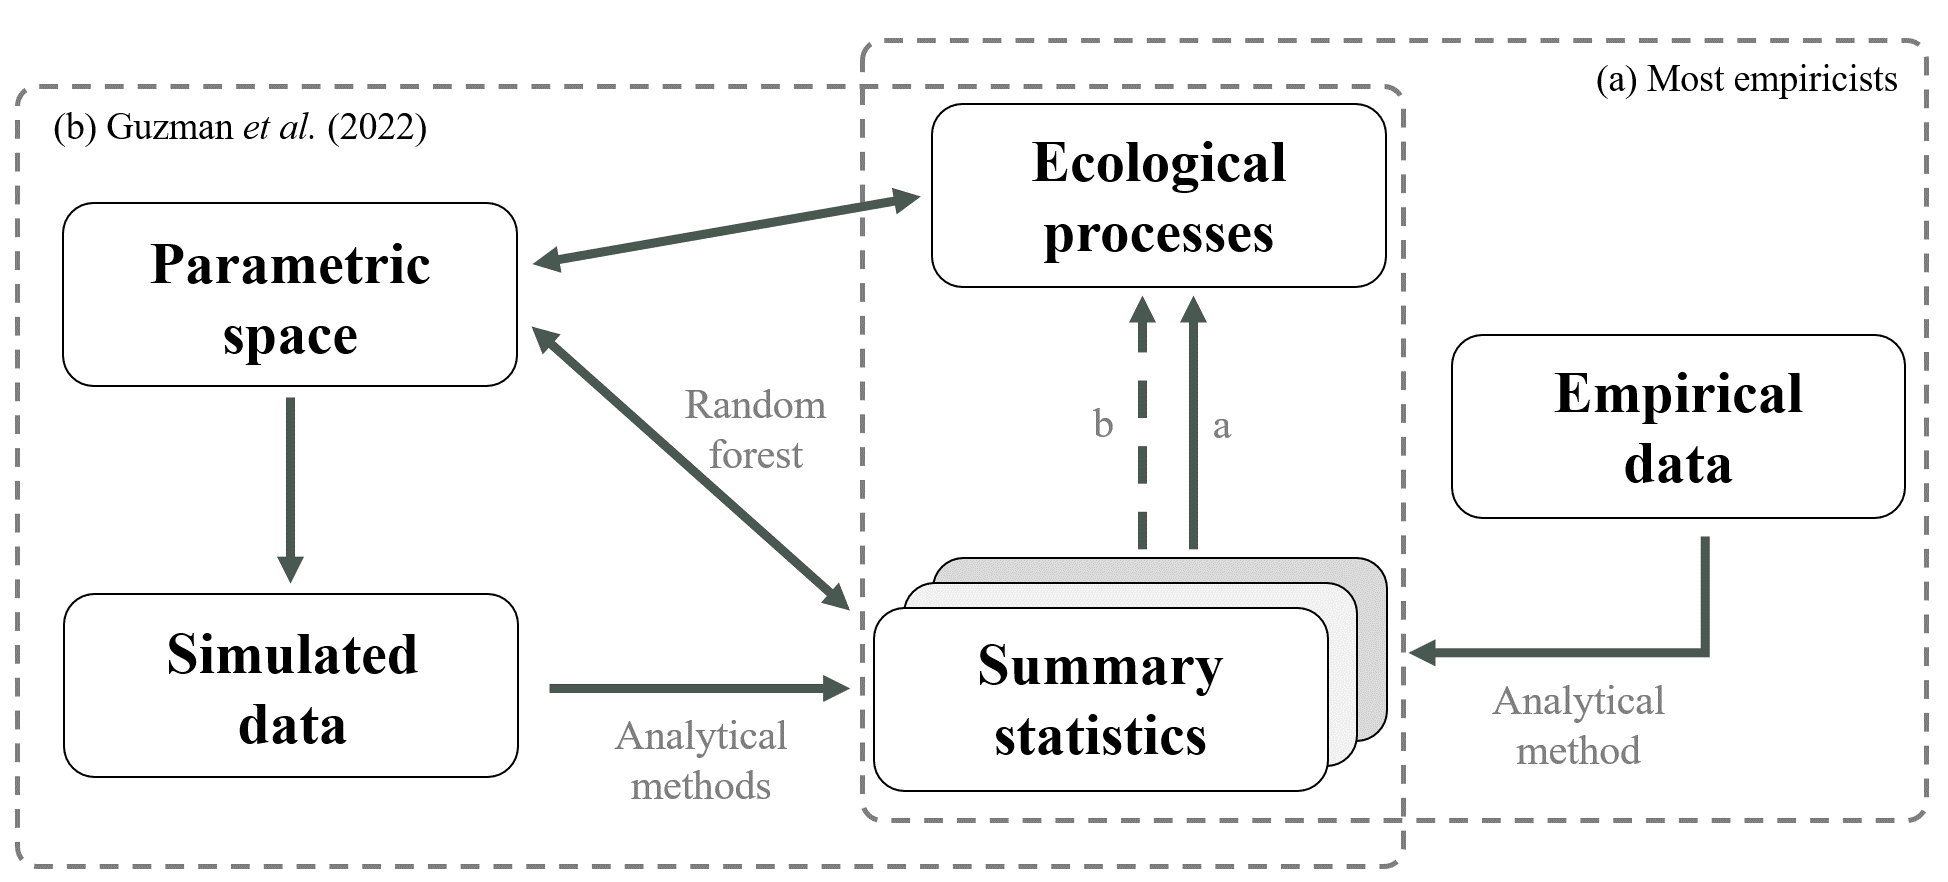
\includegraphics[width=\linewidth]{./figures/ppt/framework.png}
		\caption[Difference between the path most empiricists would take with the path proposed by \citet{guzman2022accounting}.]{\small
			Flow diagram, showing the difference between the path most empiricists would take (box at the right side), compared to the path proposed by \citet{guzman2022accounting} (box b at the left side). (a) Most empiricists disentangle the ecological processes underlying the observed metacommunities based on the summary statistics calculated by single analytical method. For example, beta-diversity is one of the analytical methods to quantify the relative importance of environmental filtering and dispersal on species turnover based on the explained variations in constrained ordination. (b) \citet{guzman2022accounting} extended this process by linking multiple summary statistics derived from different analytical methods to the parametric space of the process-based simulation model. The model parameters that regulate the strength of the ecological processes may be predicted based on the summary statistics derived from the observational data.}
		\label{fig:framework}
	\end{figure}

	Despite these analytical methods being widely used in ecological studies, ecologists have no consensus on which analytical methods can best disentangle the ecological processes underlying the observed metacommunity. This disagreement may be caused by several reasons. One is the complex interrelated effects of the ecological processes on species turnover. For example, it has been shown that the different relative importance of niche and neutral processes may result in a similar pattern in species abundance \citep{chave2002comparing, mcgill2010towards}. Therefore, we may not be successful in disentangling the underlying processes if we only consider species abundance data. The divergence/convergence of trait was also reported to frequently fail in identifying the effect of competition and environmental filtering \citep{mayfield2010opposing}. Second is the lack of comprehensive studies that synthesize or compare the performance of different analytical methods. Even though their performance has independently been assessed \citep{mcgill2006empirical, vellend2014assessing, tucker2016differentiating, ning2019general}, and criticized \citep{smith2010variation, molina2020difficulties, brown2017making}, these analytical methods have not been compared systematically. Moreover, the lack of experimental studies which control the strength of multiple processes and generate replicates of experimental metacommunities may also limit the way to evaluate these analytical methods. 
	
	\citet{guzman2022accounting} is one of the studies that attempt to synthesize multiple analytical methods to understand the underlying ecological processes (Fig. \ref{fig:framework}b). By using the simulated metacommunity data with controlled strength of the ecological processes, the performance of a single analytical method was evaluated. The authors also showed that no single analytical method had an outstanding performance in predicting the underlying ecological processes and proposed that multiple analytical methods should be considered simultaneously. However, even though \citet{guzman2022accounting} successfully integrated multiple analytical methods, the authors did not discuss whether their framework could be applied to observational data.
	
	In our study, we proposed that \citeauthor{guzman2022accounting}'s framework could be applied to observational data and understand the underlying ecological processes. We reconstructed \citeauthor{guzman2022accounting}'s framework and illustrated its application by analyzing repeated census of woody plant species in the Fushan Forest Dynamics Plot. The performance and the robustness of this framework were evaluated based on the simulated data. The pros and cons of this framework in practice were also discussed.
	
	
	